\documentclass[aspectratio=169,11pt]{beamer}

\usetheme{Madrid}
\usecolortheme{default}
\setbeamertemplate{navigation symbols}{}
\setbeamertemplate{footline}[frame number]

\usepackage[utf8]{inputenc}
\usepackage[T1]{fontenc}
\usepackage{lmodern}
\usepackage{amsmath, amssymb, bm}
\usepackage{booktabs}
\usepackage{array}
\usepackage{graphicx}
\usepackage{tikz}
\usepackage{pgfplots}
\pgfplotsset{compat=1.18}

\definecolor{accent}{RGB}{31,78,121}
\definecolor{softgray}{RGB}{88,88,88}
\definecolor{lightblue}{RGB}{232,240,249}

\setbeamercolor{title}{fg=accent}
\setbeamercolor{frametitle}{fg=accent}
\setbeamercolor{structure}{fg=accent}
\setbeamercolor{block title}{fg=white,bg=accent}
\setbeamercolor{block body}{bg=lightblue}
\setbeamercolor{normal text}{fg=softgray}

\title{Dynamic Programming and Markov Decision Processes}
\subtitle{A Coherent Algorithmic Story with Financial Examples}
\author{Group 6: Feiyang Liu, Zhesheng Xu, Minghao Tang}
\date{April 2026}
\institute{Algorithm Analysis Presentation}

\begin{document}

\begin{frame}
  \titlepage
\end{frame}

\begin{frame}{Presentation Roadmap}
  \tableofcontents
\end{frame}

\section{Why This Topic}

\begin{frame}{Motivation}
  \begin{itemize}
    \item Many decision problems combine two difficulties: sequential choices and uncertainty.
    \item Dynamic programming provides the computational principle: solve a large problem by solving smaller ones.
    \item Markov models provide the probabilistic principle: the current state is sufficient for future prediction.
    \item Markov decision processes connect both ideas into one optimization framework.
  \end{itemize}

  \vspace{0.4cm}
  \begin{block}{Core message}
    Once the problem is written as states, actions, transitions, and rewards, Bellman recursion turns planning into a sequence of local updates.
  \end{block}
\end{frame}

\section{From Dynamic Programming to MDPs}

\begin{frame}{Dynamic Programming in One Slide}
  \begin{columns}[T]
    \column{0.54\textwidth}
    \begin{itemize}
      \item \textbf{Stage}: the time or decision index.
      \item \textbf{State}: a summary of the information that matters now.
      \item \textbf{Decision}: the action chosen in that state.
      \item \textbf{Value function}: the best attainable objective from that state onward.
    \end{itemize}

    \column{0.42\textwidth}
    \begin{block}{Two structural conditions}
      \begin{itemize}
        \item Optimal substructure
        \item No aftereffect
      \end{itemize}
    \end{block}
  \end{columns}

  \vspace{0.3cm}
  \[
    V_k(s) = \max_{a \in \mathcal{A}(s)} \left\{ r_k(s,a) + V_{k+1}(T(s,a)) \right\}
  \]
\end{frame}

\begin{frame}{Why Markov Structure Matters}
  \begin{itemize}
    \item A stochastic process is Markov if the next state depends only on the current state.
    \item This property is exactly what makes dynamic programming feasible under uncertainty.
    \item The transition matrix \(P\) summarizes all one-step state dynamics.
  \end{itemize}

  \[
    \Pr(X_{t+1}=j \mid X_t=i, X_{t-1}, \dots, X_0)
    =
    \Pr(X_{t+1}=j \mid X_t=i)
  \]

  \begin{block}{Interpretation}
    The state is not just a label. It is the information set that makes the future conditionally independent of the past.
  \end{block}
\end{frame}

\begin{frame}{Markov Decision Process Formulation}
  \begin{columns}[T]
    \column{0.52\textwidth}
    \begin{itemize}
      \item State space: \(\mathcal{S}\)
      \item Action space: \(\mathcal{A}\)
      \item Transition kernel: \(P(s' \mid s,a)\)
      \item Reward function: \(r(s,a)\) or \(r(s,a,s')\)
      \item Discount factor: \(\gamma \in [0,1)\)
    \end{itemize}

    \column{0.44\textwidth}
    \begin{block}{Policy}
      A policy \(\pi(a \mid s)\) specifies how actions are selected in each state.
    \end{block}
  \end{columns}

  \vspace{0.2cm}
  \[
    G_t = \sum_{k=0}^{\infty} \gamma^k R_{t+k+1}
  \]
\end{frame}

\begin{frame}{Bellman Expectation and Optimality Equations}
  \begin{align*}
    V^{\pi}(s)
    &=
    \sum_{a} \pi(a \mid s)
    \sum_{s'} P(s' \mid s,a)
    \left[r(s,a,s') + \gamma V^{\pi}(s')\right] \\
    V^*(s)
    &=
    \max_{a}
    \sum_{s'} P(s' \mid s,a)
    \left[r(s,a,s') + \gamma V^*(s')\right]
  \end{align*}

  \begin{itemize}
    \item The expectation equation evaluates a fixed policy.
    \item The optimality equation replaces averaging over actions with maximization.
    \item This is the mathematical bridge from modeling to computation.
  \end{itemize}
\end{frame}

\section{Algorithms}

\begin{frame}{Two Standard Dynamic Programming Algorithms}
  \begin{columns}[T]
    \column{0.49\textwidth}
    \begin{block}{Policy iteration}
      \begin{enumerate}
        \item Start from a policy \(\pi\)
        \item Evaluate \(V^{\pi}\)
        \item Improve greedily with respect to \(V^{\pi}\)
        \item Repeat until the policy stops changing
      \end{enumerate}
    \end{block}

    \column{0.49\textwidth}
    \begin{block}{Value iteration}
      \begin{enumerate}
        \item Start from an initial value estimate
        \item Apply Bellman optimality updates
        \item Stop when updates become negligible
        \item Recover the greedy policy
      \end{enumerate}
    \end{block}
  \end{columns}

  \vspace{0.2cm}
  \[
    V_{k+1}(s) = \max_{a} \sum_{s'} P(s' \mid s,a)\left[r(s,a,s') + \gamma V_k(s')\right]
  \]
\end{frame}

\begin{frame}{Computational Perspective}
  \begin{itemize}
    \item For a finite MDP with \(|\mathcal{S}|\) states and \(|\mathcal{A}|\) actions:
  \end{itemize}

  \[
    \text{One Bellman sweep} = \mathcal{O}(|\mathcal{S}|^2 |\mathcal{A}|)
  \]

  \[
    \text{Value iteration total} = \mathcal{O}(K |\mathcal{S}|^2 |\mathcal{A}|)
  \]

  \[
    \text{Exact linear-system policy evaluation} = \mathcal{O}(|\mathcal{S}|^3)
  \]

  \begin{block}{Practical takeaway}
    Dynamic programming is attractive when the state space is moderate and the model is explicit. It becomes difficult when the state space is large or continuous.
  \end{block}
\end{frame}

\section{Example 1: Trading MDP}

\begin{frame}{Example 1: A Two-State Trading MDP}
  \begin{columns}[T]
    \column{0.55\textwidth}
    \begin{itemize}
      \item States: \(s_1=\) Bull, \(s_2=\) Bear
      \item Actions: Buy or Sell
      \item Discount factor: \(\gamma = 0.9\)
      \item The example is intentionally simple so that the algorithmic logic is transparent
    \end{itemize}

    \column{0.42\textwidth}
    \begin{block}{Question}
      Which action is optimal in each market regime once immediate payoff and expected future value are combined?
    \end{block}
  \end{columns}
\end{frame}

\begin{frame}{Reward Structure and Transition Logic}
  \begin{columns}[T]
    \column{0.42\textwidth}
    \begin{table}
      \centering
      \begin{tabular}{lcc}
        \toprule
        State & Buy & Sell \\
        \midrule
        Bull & 10 & -5 \\
        Bear & -10 & 5 \\
        \bottomrule
      \end{tabular}
    \end{table}

    \begin{itemize}
      \item Momentum favors Buy in Bull.
      \item Downside control favors Sell in Bear.
      \item Future transitions still matter.
    \end{itemize}

    \column{0.54\textwidth}
    \begin{center}
      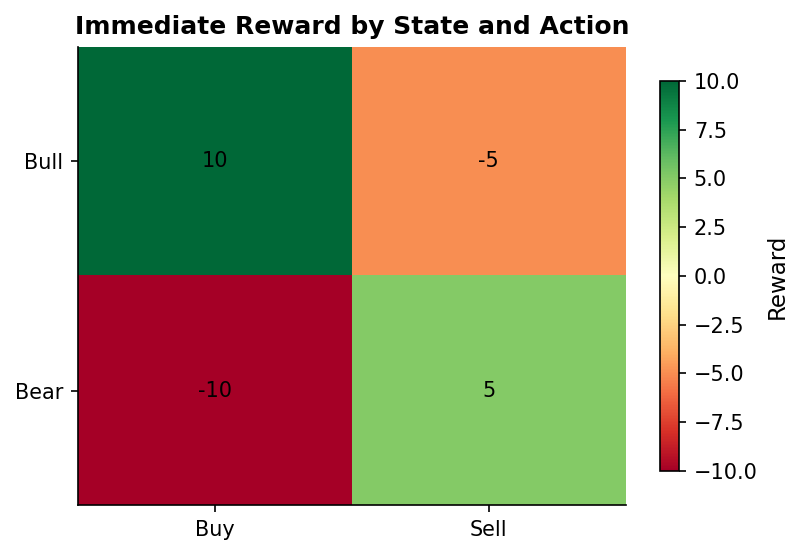
\includegraphics[width=\linewidth]{../assets/figures/trading_reward_heatmap.png}
    \end{center}
  \end{columns}
\end{frame}

\begin{frame}{Algorithmic Result for the Trading Example}
  \begin{columns}[T]
    \column{0.46\textwidth}
    \begin{block}{Optimal policy}
      \[
        \pi^*(\text{Bull}) = \text{Buy}, \qquad
        \pi^*(\text{Bear}) = \text{Sell}
      \]
    \end{block}

    \begin{block}{Optimal values}
      \[
        V^*(\text{Bull}) = 86.50, \qquad
        V^*(\text{Bear}) = 81.50
      \]
    \end{block}

    \column{0.50\textwidth}
    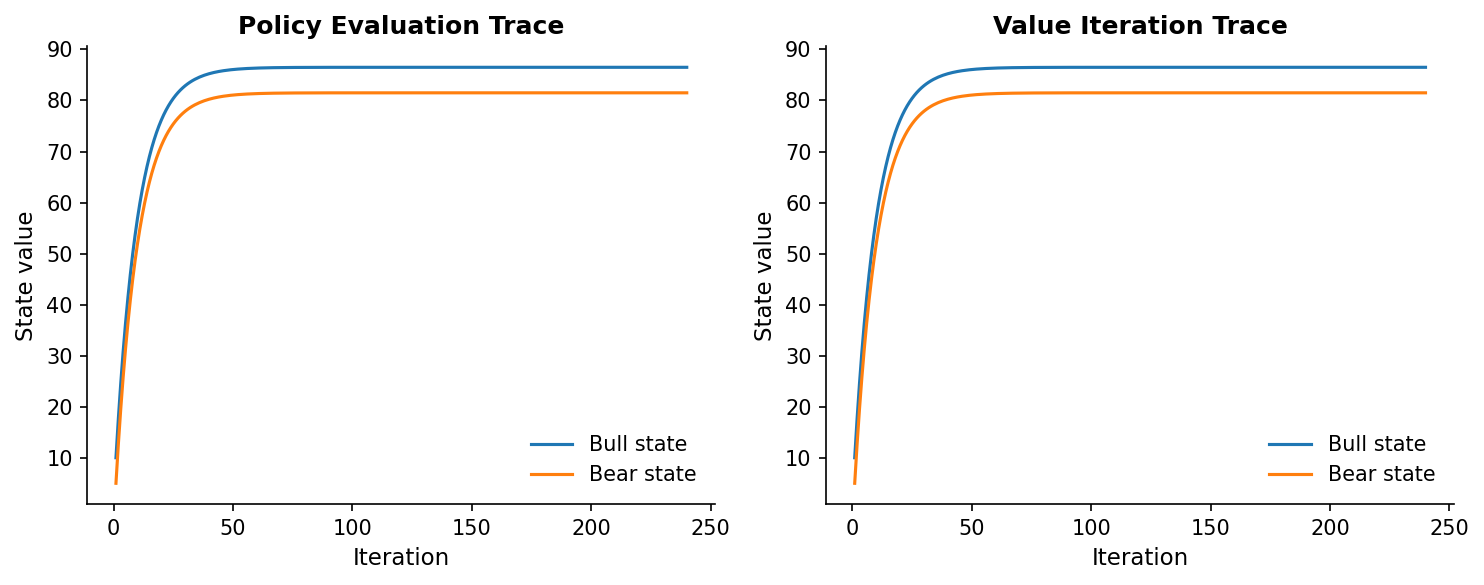
\includegraphics[width=\linewidth]{../assets/figures/trading_convergence.png}
  \end{columns}
\end{frame}

\section{Example 2: American Put Option}

\begin{frame}{Why an American Put Fits Dynamic Programming}
  \begin{itemize}
    \item At each node, the holder must choose between \textbf{exercise now} and \textbf{continue holding}.
    \item That is a sequential decision problem under uncertainty.
    \item The continuation value depends on the next-period option values, so backward induction is the natural dynamic programming method.
  \end{itemize}

  \[
    V_t(S_t)=\max \left\{ K-S_t,\ e^{-r\Delta t}\left[pV_{t+1}(S_tu) + (1-p)V_{t+1}(S_td)\right] \right\}
  \]
\end{frame}

\begin{frame}{Model Setup}
  \begin{table}
    \centering
    \begin{tabular}{lc}
      \toprule
      Parameter & Value \\
      \midrule
      Initial stock price \(S_0\) & 100 \\
      Strike price \(K\) & 95 \\
      Maturity & 3 months \\
      Number of steps & 3 \\
      Annual rate \(r\) & 12\% \\
      Volatility \(\sigma\) & 20\% \\
      \bottomrule
    \end{tabular}
  \end{table}

  \begin{block}{Decision rule}
    Exercise when intrinsic value exceeds continuation value; otherwise hold.
  \end{block}
\end{frame}

\begin{frame}{Backward-Induction Result}
  \begin{columns}[T]
    \column{0.37\textwidth}
    \begin{itemize}
      \item Early exercise appears only in the lowest price branch.
      \item Earlier nodes are worth holding.
      \item The initial option value is \(V_0 = 1.18\).
    \end{itemize}

    \begin{block}{Interpretation}
      Backward induction compares immediate exercise with discounted continuation at every node.
    \end{block}

    \column{0.59\textwidth}
    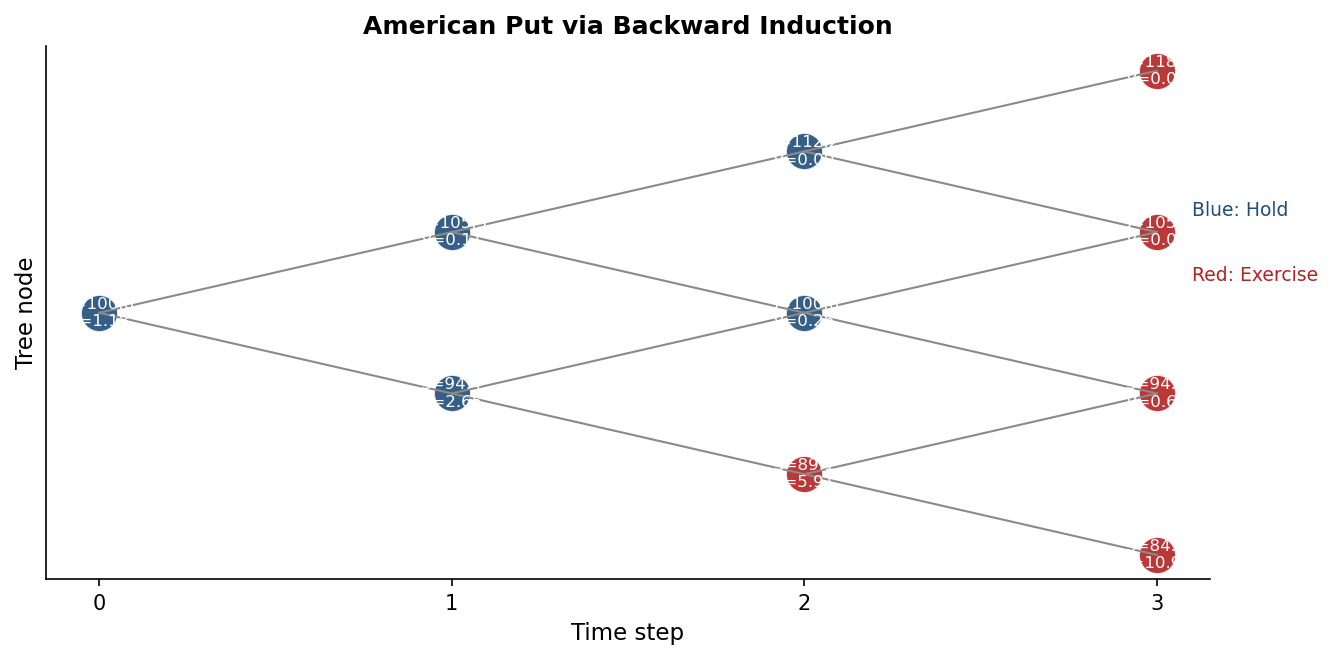
\includegraphics[width=\linewidth]{../assets/figures/american_put_tree.png}
  \end{columns}
\end{frame}

\section{Takeaways}

\begin{frame}{Main Conclusions}
  \begin{itemize}
    \item Dynamic programming is the computational engine behind many sequential optimization problems.
    \item Markov structure is what makes the recursion tractable: the state compresses the relevant information.
    \item Bellman equations unify evaluation, optimization, and algorithm design.
    \item Even simple financial examples show the full logic clearly: policy choice in an MDP and exercise choice in an American option.
  \end{itemize}
\end{frame}

\begin{frame}{End}
  \centering
  {\Large Thank you.}

  \vspace{0.4cm}
  Questions and discussion.
\end{frame}

\end{document}
